% !TEX root = ../agglo_clust_review.tex

\begin{figure}[t]
\centering
% 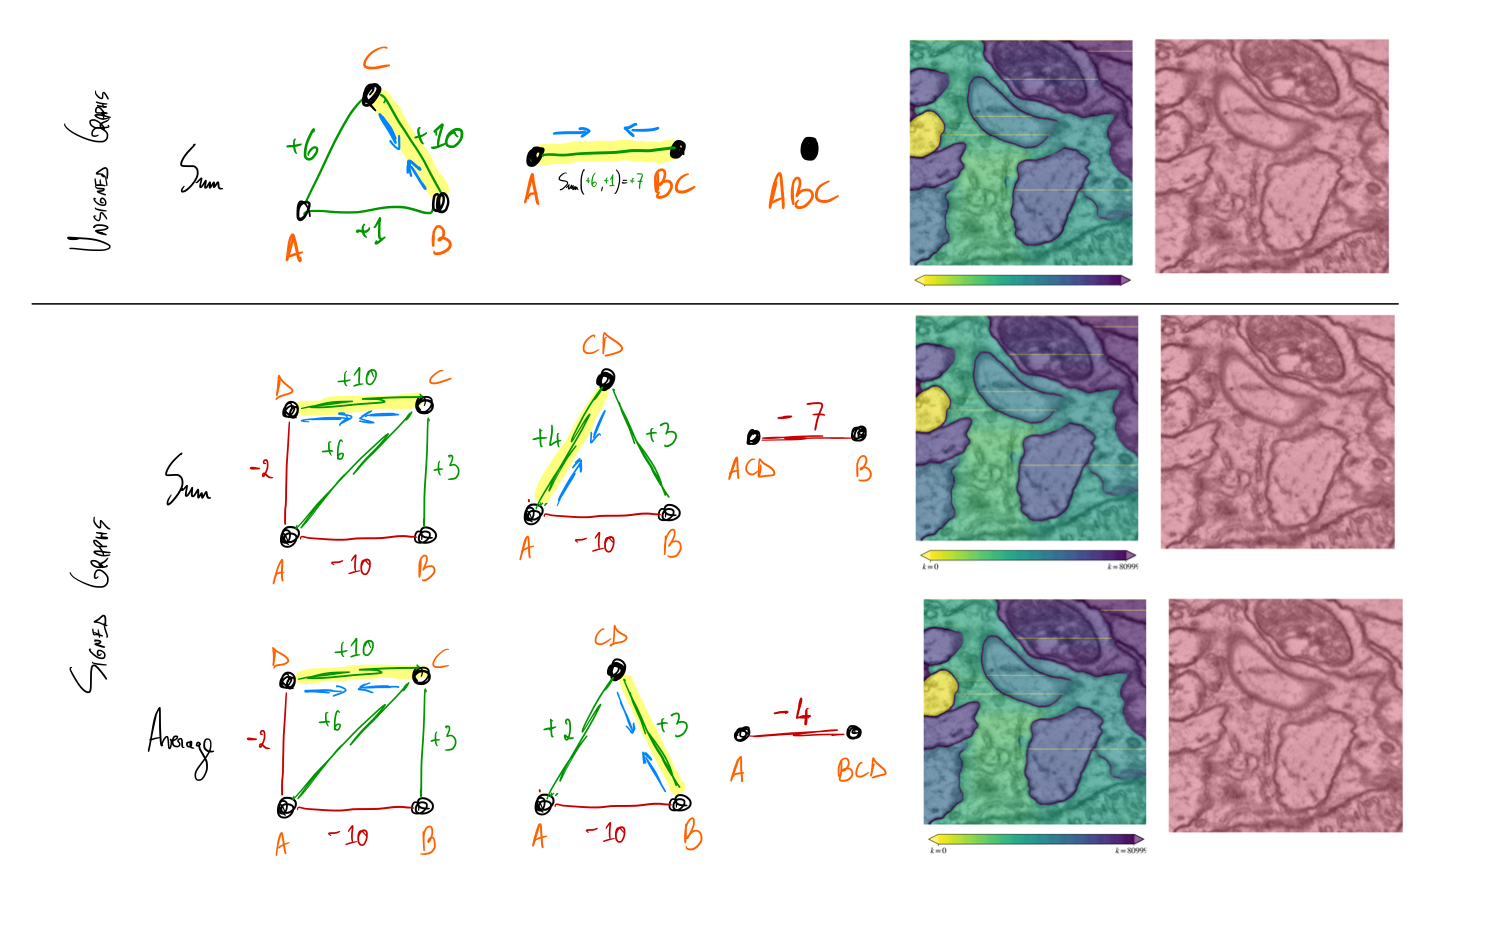
\includegraphics[width=0.5\textwidth,trim=0.4in 1.2in 0.in 0.05in,clip]{./figs/intro_image.jpg} % left bottom right top
\includegraphics[width=\textwidth]{./figs/comparison.pdf} % left bottom right top
\caption{
{\small Comparison of results from different update rules on signed graph with and without cannot-link constraints 
}
 % main ideas and contributions
\label{fig:cremi_comparison}}
\end{figure}
\begin{figure}[b]
\centering
% 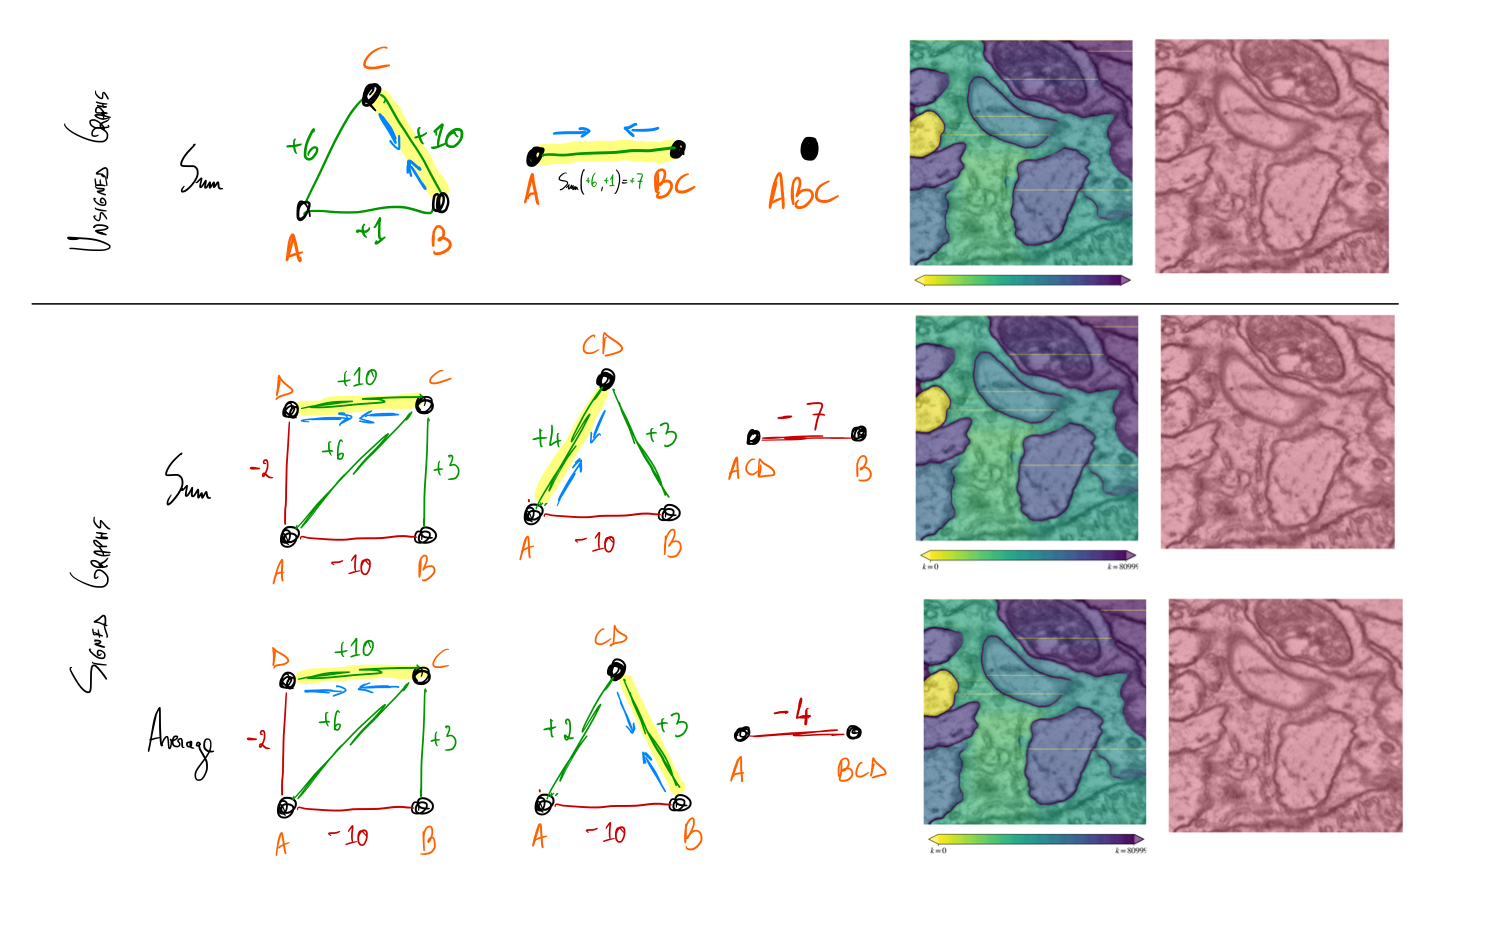
\includegraphics[width=0.5\textwidth,trim=0.4in 1.2in 0.in 0.05in,clip]{./figs/intro_image.jpg} % left bottom right top
\includegraphics[width=\textwidth]{./figs/cityscapes_compare.pdf} % left bottom right top
\caption{
{\small Comparison of results from different update rules on signed graph with and without cannot-link constraints 
}
 % main ideas and contributions
\label{fig:cytiscapes_comparison}}
\end{figure}

% \begin{figure}
% \centering
%         \begin{subfigure}[t]{0.46 \linewidth}
%         \centering
%         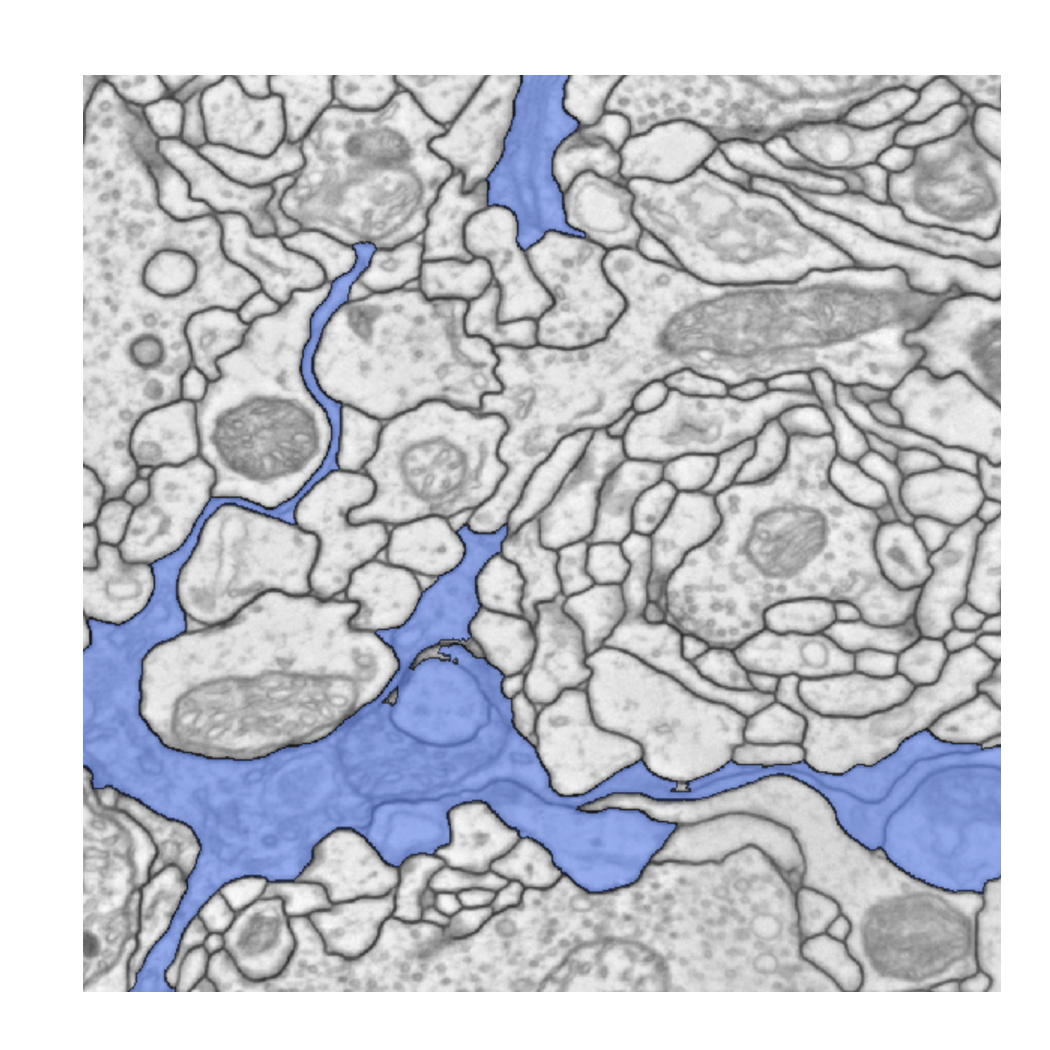
\includegraphics[width=0.98\textwidth]{figs/comparison/sum_F.pdf}
%         % \caption{Thresholding of local boundary maps ~(THRESH)} \label{fig:thresh}
%     \end{subfigure}%
%     \begin{subfigure}[t]{0.46 \linewidth}
%         \centering
%         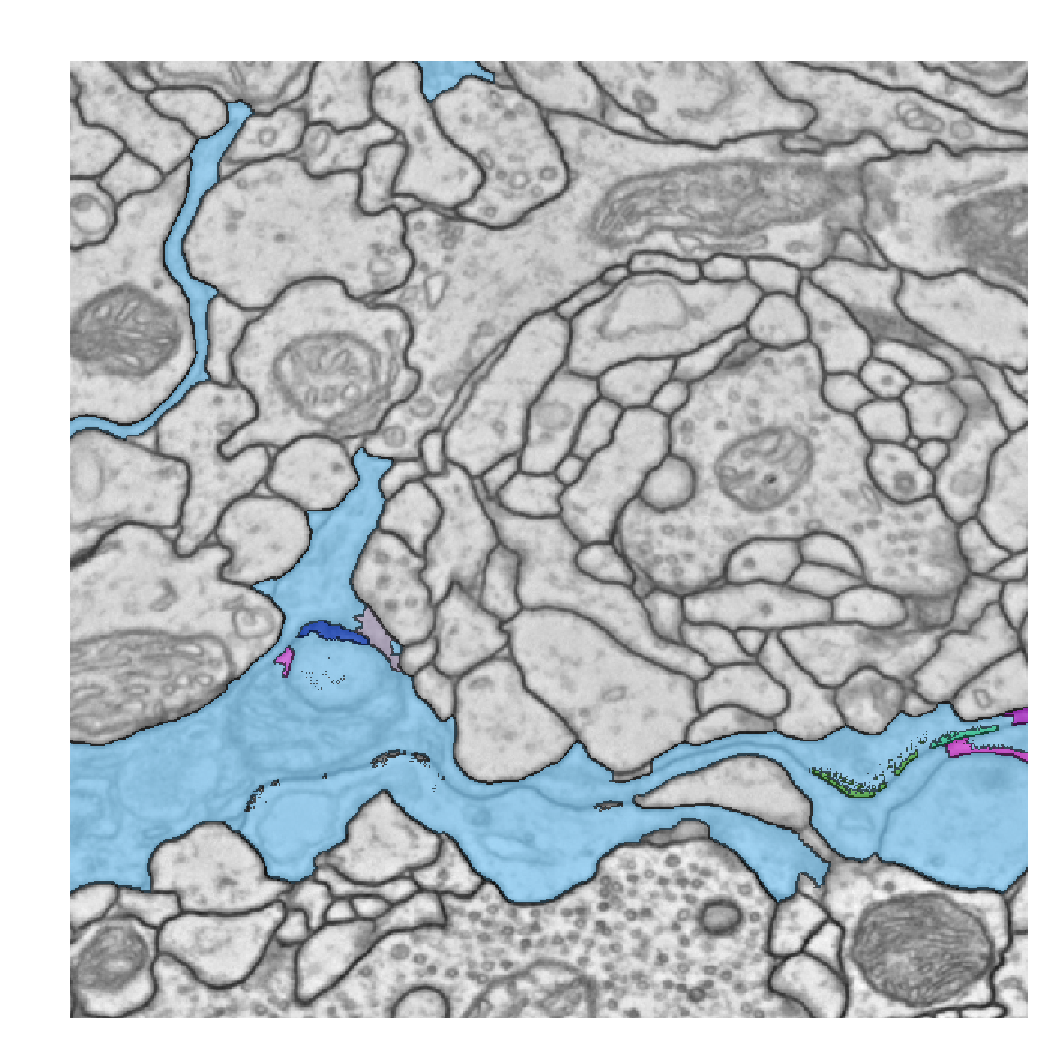
\includegraphics[width=0.98\textwidth]{figs/comparison/sum_T.pdf}
%         % \caption{Watershed, seeded at local minima of the smoothed input map~(WS)} \label{fig:ws}
%     \end{subfigure}\hspace{0.5cm}%

%     % \vspace{0.3cm}
%     \begin{subfigure}[t]{0.92 \linewidth}
%         \centering
%         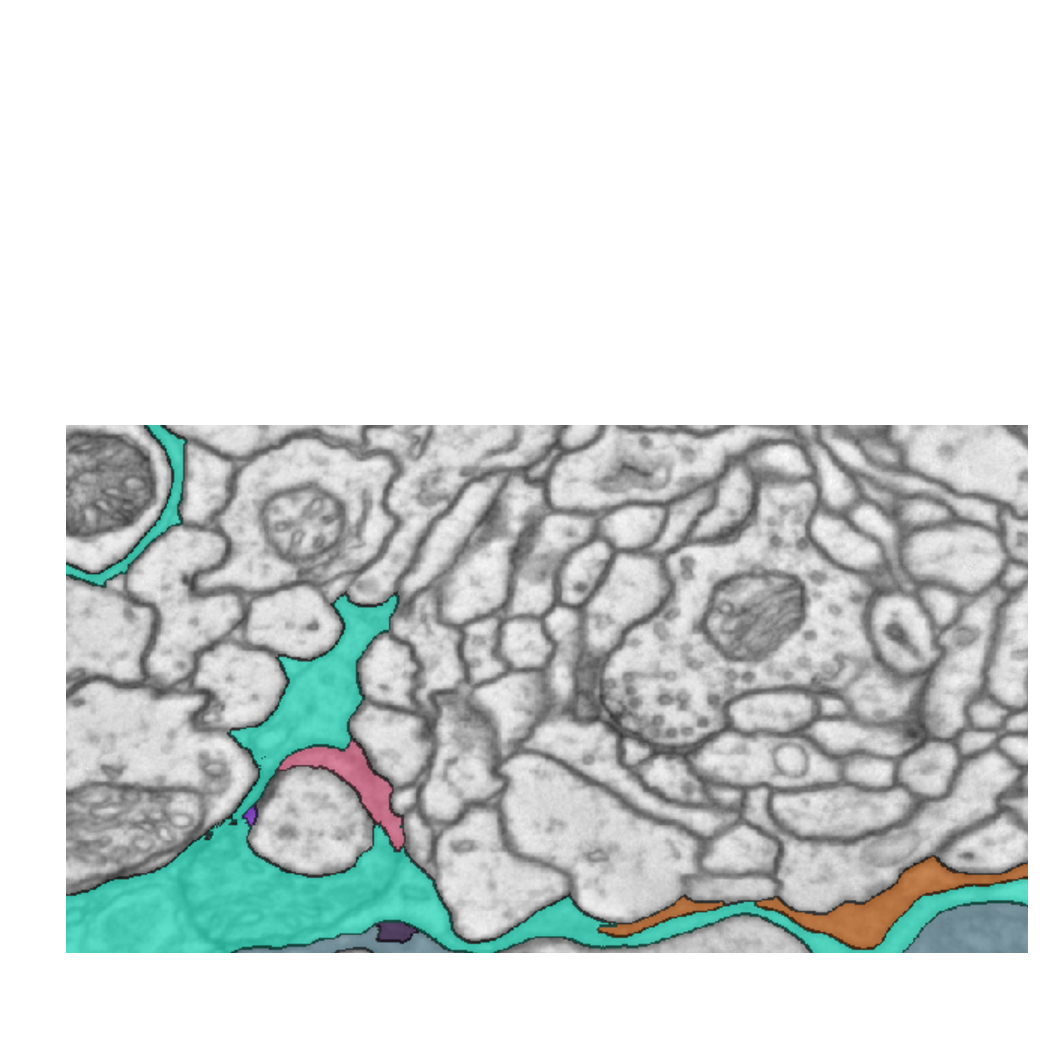
\includegraphics[width=1.\textwidth]{figs/comparison/MWS.pdf}
%         % \caption{Multicut partitioning based segmentation~(MC-FULL)} \label{fig:mc_full}
%     \end{subfigure}\hspace{0.5cm}

%     \begin{subfigure}[t]{0.46 \linewidth}
%         \centering
%         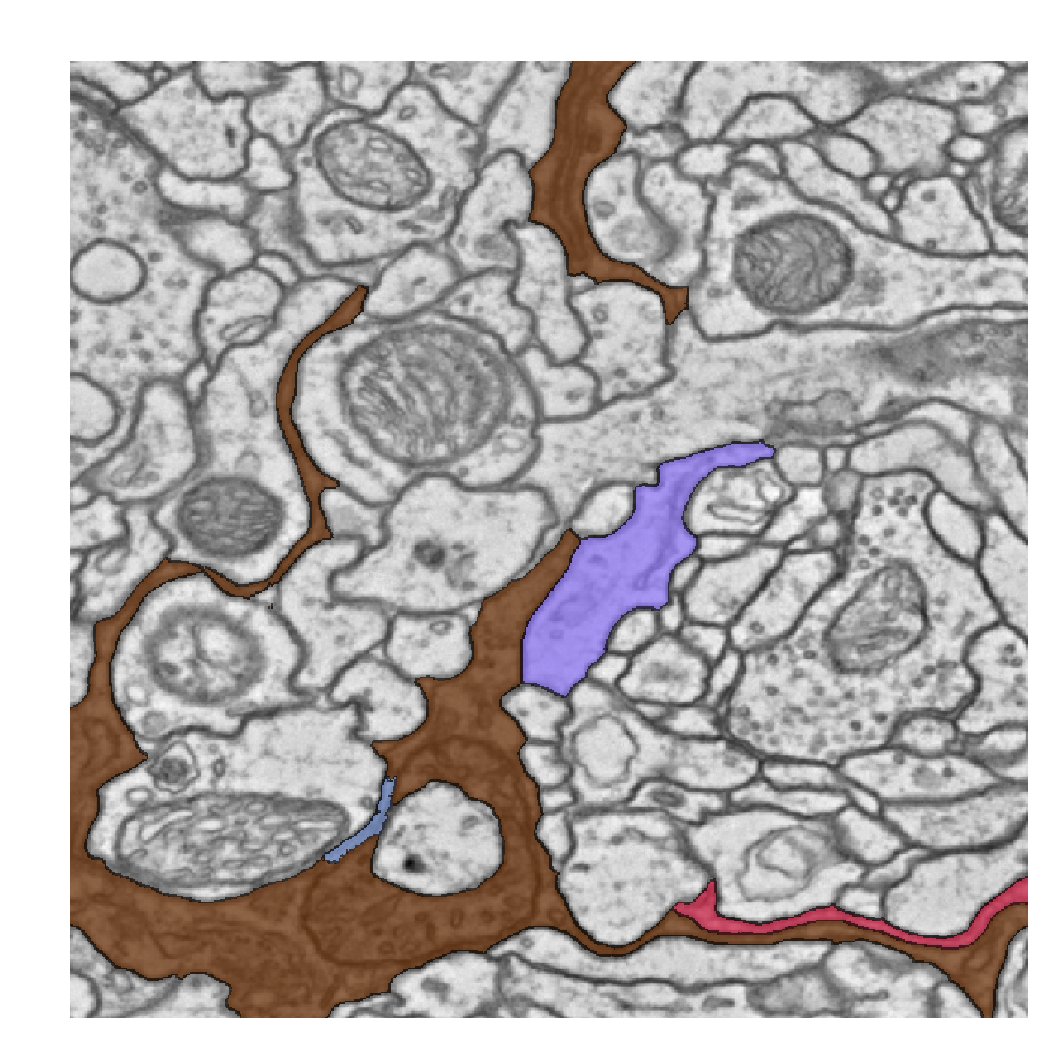
\includegraphics[width=0.98\textwidth]{figs/comparison/mean_F.pdf}
%         % \caption{Thresholding of local boundary maps ~(THRESH)} \label{fig:thresh}
%     \end{subfigure}%
%     \begin{subfigure}[t]{0.46 \linewidth}
%         \centering
%         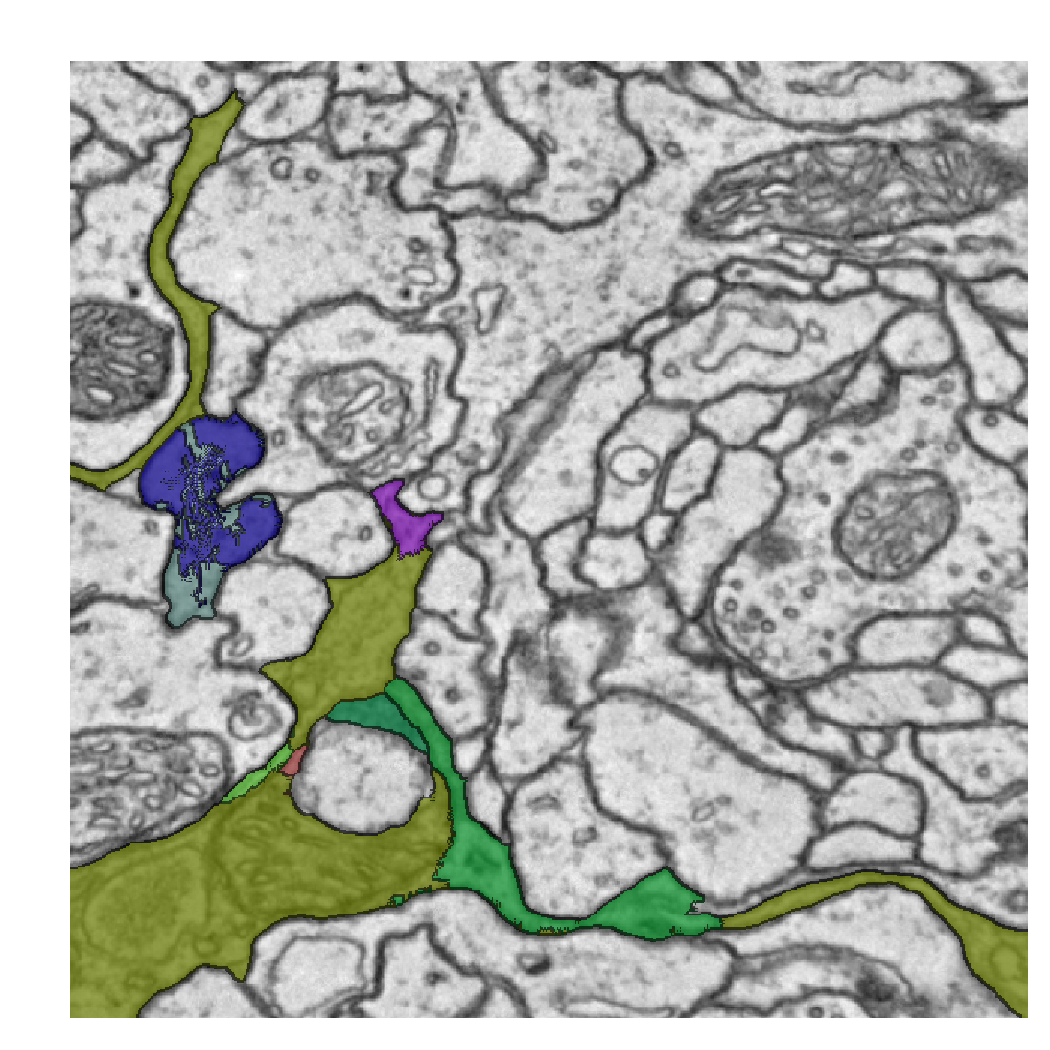
\includegraphics[width=0.98\textwidth]{figs/comparison/mean_T.pdf}
%         % \caption{Watershed, seeded at local minima of the smoothed input map~(WS)} \label{fig:ws}
%     \end{subfigure}\hspace{0.5cm}%

% \begin{subfigure}[t]{0.46 \linewidth}
%         \centering
%         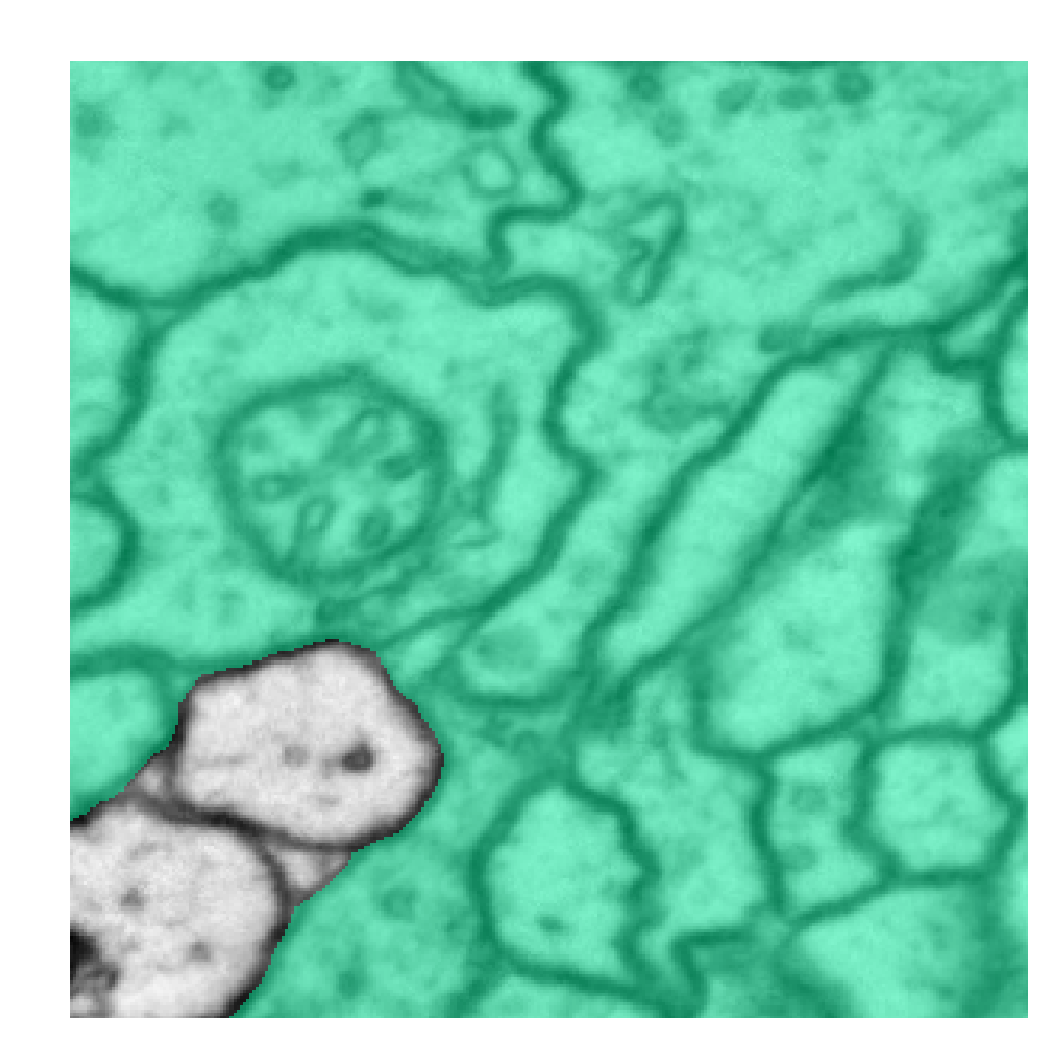
\includegraphics[width=0.98\textwidth]{figs/comparison/max_F.pdf}
%         % \caption{Thresholding of local boundary maps ~(THRESH)} \label{fig:thresh}
%     \end{subfigure}%
%     \begin{subfigure}[t]{0.46 \linewidth}
%         \centering
%         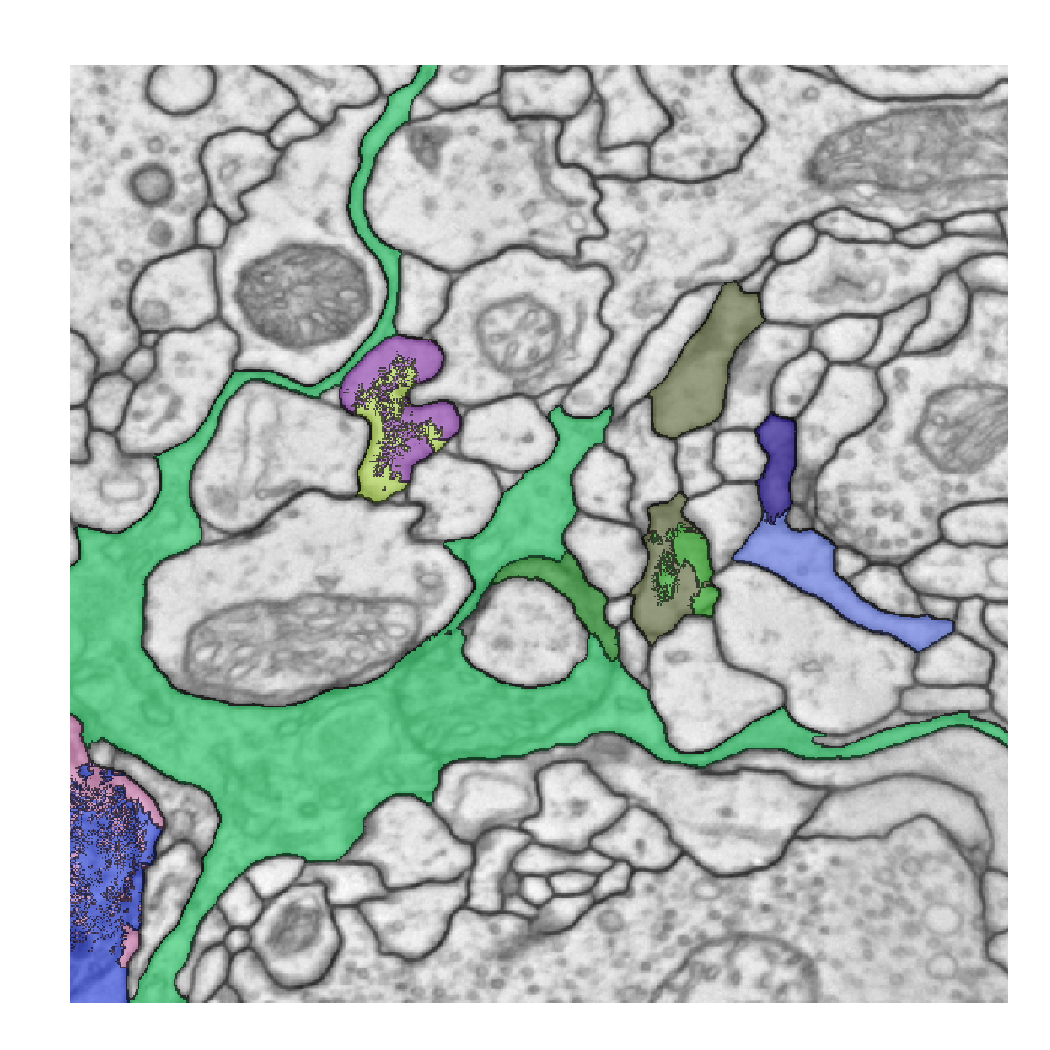
\includegraphics[width=0.98\textwidth]{figs/comparison/max_T.pdf}
%         % \caption{Watershed, seeded at local minima of the smoothed input map~(WS)} \label{fig:ws}
%     \end{subfigure}\hspace{0.5cm}%

% \begin{subfigure}[t]{0.46 \linewidth}
%         \centering
%         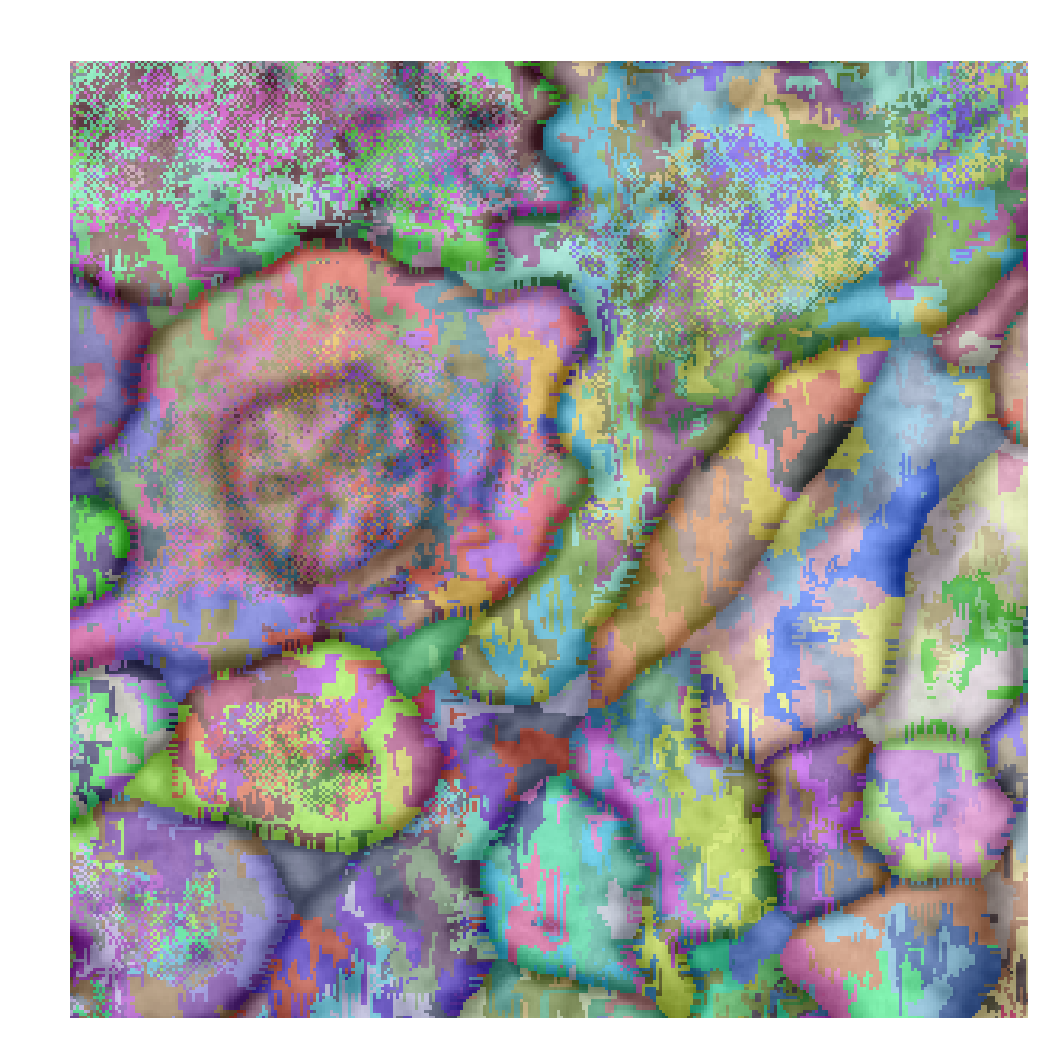
\includegraphics[width=0.98\textwidth]{figs/comparison/min_F.pdf}
%         % \caption{Thresholding of local boundary maps ~(THRESH)} \label{fig:thresh}
%     \end{subfigure}%
%     \begin{subfigure}[t]{0.46 \linewidth}
%         \centering
%         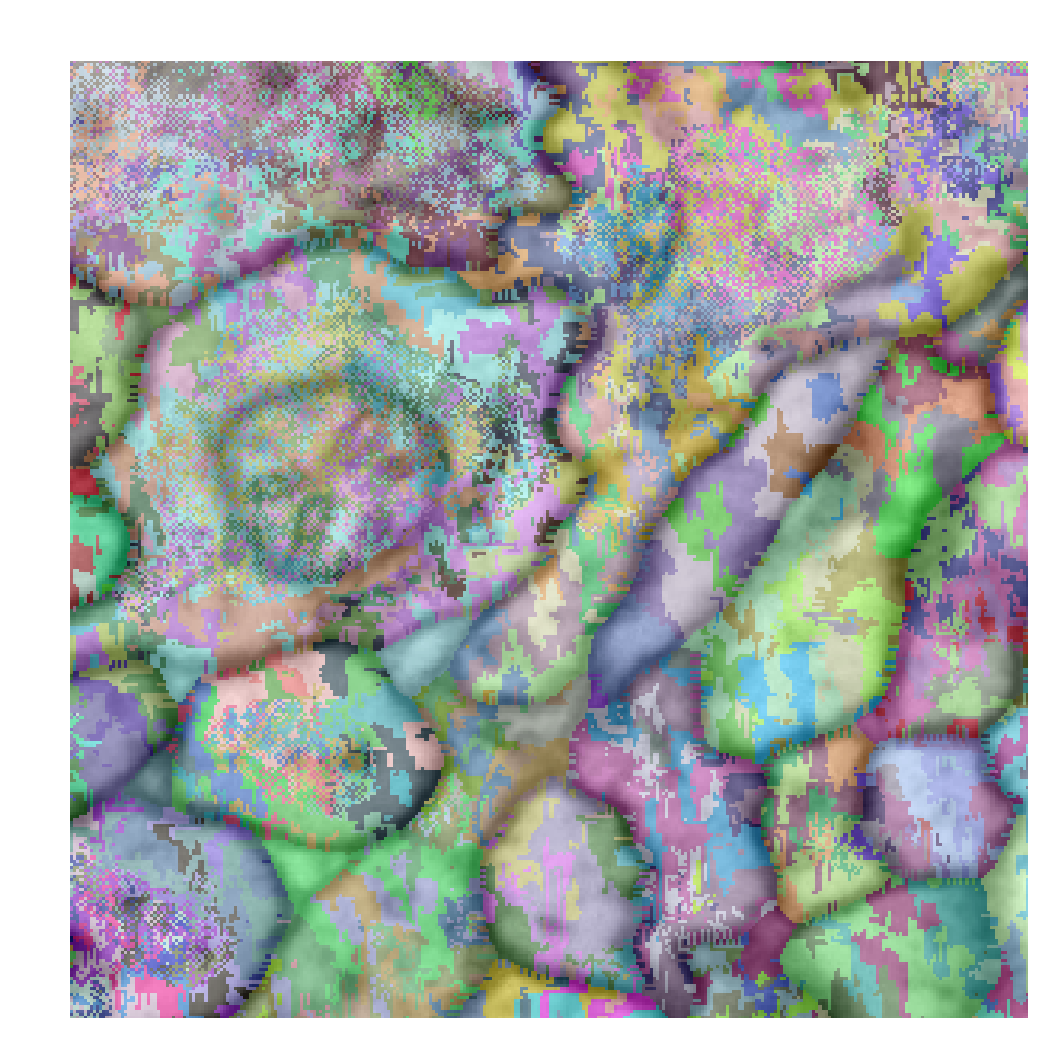
\includegraphics[width=0.98\textwidth]{figs/comparison/min_T.pdf}
%         % \caption{Watershed, seeded at local minima of the smoothed input map~(WS)} \label{fig:ws}
%     \end{subfigure}\hspace{0.5cm}%

%     % \vspace{-0.4cm}
%     \caption{Comparison of results from different update rules on signed graph with and without cannot-link constraints \TODO{add arrows/circles highlighting merge/split mistakes and correct decisions. Align; add captions}}
%     \label{fig:isbi-examples}
% \end{figure}% \captionsetup[


\subsection{Evaluating different update rules} \label{sec:exp_first_comparison}
\begin{itemize}
  \item Highlight difference of the sum in Fig. \ref{fig:intro_figure}
  % \item compare different choices of signed-cost-mappings (say which one worked best)
  \item present cremi crop-C table and rule out single and complete linkage
\end{itemize}

Among the update rules listed in Table \ref{tab:linkage-criteria}, in the next sections we will only focus on \emph{sum}, \emph{arithmetic mean} and \emph{absolute maximum}, since they performed best in these experiments.


